% =========================================================================== %

\begin{frame}[t,plain]
\titlepage
\end{frame}

% =========================================================================== %

\begin{frame}{Recap}
%
\begin{columns}[T]
\column{.5\linewidth}
\begin{itemize}
\item Constants module \texttt{scipy.constants}
	\begin{itemize}
	\item Direct Constants and Lookup Functions
	\end{itemize}
\item Special functions module  \texttt{scipy.specials}
\item Numerical Integration from \texttt{scipy.integrate}
	\begin{itemize}
	\item \texttt{quad}, \texttt{dblquad} and \texttt{tplquad} -- general purpose integrators
	\item Vector integration -- use of pre-computed values
	\item Trapeze, Simpson, Romberg
	\end{itemize}
\end{itemize}
%
\column{.5\linewidth}
\begin{itemize}
\item Curve Fitting from \texttt{scipy.optimize}
	\begin{itemize}
	\item \texttt{curve\_fit} returns \inPy{tuple}: Fit results and covariance
	\item Sometimes only works if a \enquote{good guess} is provided
	\end{itemize}
\item Fourier Transform from \texttt{scipy.fft}
	\begin{itemize}
	\item Rescaling might be necessary
	\item Numerical errors due to finite resolution
	\end{itemize}
\item Differential Equations with \texttt{scipy.integrate}
	\begin{itemize}
	\item Actually only numerical integration
	\item \texttt{odeint}
	\item Differential equation in a function
	\item Returns: matrix of first $n$ derivatvives
	\end{itemize}
\end{itemize}

\end{columns}
%
\begin{center}
	\emph{Any Questions?}
\end{center}
%
\end{frame}

% =========================================================================== %

\begin{frame}
%
\begin{columns}[T]
\column{.5\linewidth}
\begin{center}
	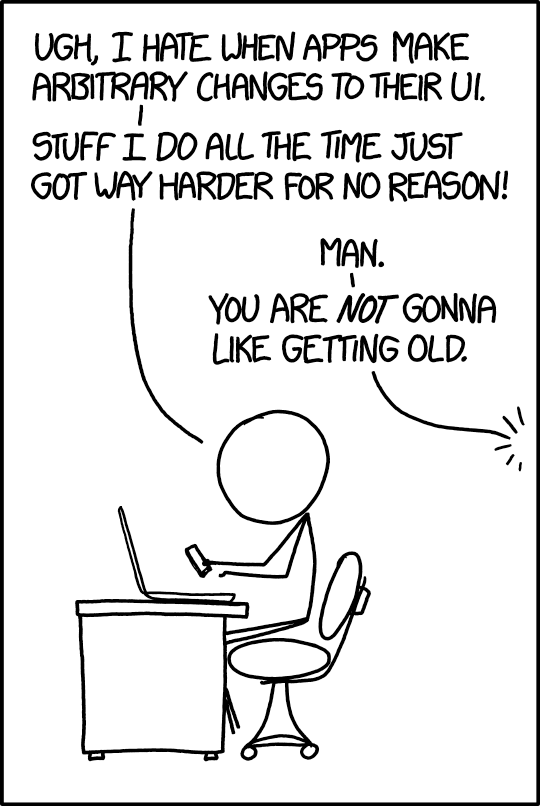
\includegraphics[width=.67\linewidth]{./gfx/xkcd-change}
\end{center}
%
\column{.5\linewidth}
\begin{Large}
	{UI Change}
\end{Large}
%
\begin{center}
	\vspace{60pt}
	\emph{I know they said this change is permanent, but surely when they hear how much we're complaining someone will find a way to change things back.}

	\vspace{6pt}
	Source: \url{https://xkcd.com/1770/}
\end{center}
\end{columns}

%
\end{frame}

% =========================================================================== %\\

\begin{frame}{tkInter -- Graphical User Interfaces with TK}
%
\begin{itemize}
\item GUI toolkit shipped with Python, works with Windows, Linux, Mac
	\begin{itemize}
	\item TK is actually a toolkit from language Tcl
	\item tkInter makes it work in Python
	\item Slightly different versions for Python3 and Python2
	\end{itemize}
\item Provides collection of \enquote{Widgets} (GUI-elements such as windows, buttons, checkbuttons, ...)
\item Logic similar to other GUI systems (\eg Qt, wxwidgets, gtk, Win32 GUI, ...)
\item Brief overview of the features: \url{https://www.tutorialspoint.com/python3/python_gui_programming.htm}
\item More complete reference: \url{https://docs.python.org/3/library/tk.html}
\item More complete tutorial: \url{https://tkdocs.com/tutorial/index.html}
\end{itemize}
%
\end{frame}

% =========================================================================== %

\begin{frame}[fragile]{A Minimal Example}
%
\begin{tcbraster}[raster columns=2,
                  raster equal height,
                  nobeforeafter,
                  raster column skip=0.5cm]
\begin{codebox}[Example: Window with tkInter]
\begin{minted}[linenos, fontsize=\scriptsize]{python3}
import tkinter as tk
top = tk.Tk()
top.title("tk")
top.mainloop()
\end{minted}
\end{codebox}
%
\begin{tcolorbox}[title=Output: Window with tkInter]
\centering
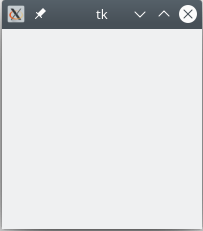
\includegraphics[width=.3\linewidth]{./gfx/tk-mini}
\end{tcolorbox}
\end{tcbraster}
%
\begin{itemize}
\item Line 1: Load Module
\item Line 2: Create (Main) Widget
\item Line 3: Set the window's title (as a stand in for fixing the properties)
\item Line 4: Pass Control to tkinter
\end{itemize}
%
\end{frame}

% =========================================================================== %

\begin{frame}{Logic and Structure}
%
\begin{itemize}
\item Object oriented approach (object \texttt{top})
\item Default Values
	\begin{itemize}
	\item Window Size, title text, position, ...
	\item[\Thus] Methods or ways to change properties
	\end{itemize}
\item Objects usually are \emph{within} each other (Button in Window)
	\begin{itemize}
	\item[\Thus] Hierarchical Principle
	\end{itemize}
\item Mainloop takes over control
	\begin{itemize}
	\item[\Thus] All definitions need to be done before call to \texttt{mainloop}
	\end{itemize}
\item Objects should be interactive
	\begin{itemize}
	\item[\Thus] Some sort of \emph{callback code}: own functions called by \texttt{mainloop}
	\end{itemize}
\end{itemize}
%
\end{frame}

% =========================================================================== %

\begin{frame}[fragile]
%
\begin{tcbraster}[raster columns=2,
                  raster equal height,
                  nobeforeafter,
                  raster column skip=0.5cm]
\begin{codebox}[Example: Hello World]
\begin{minted}[fontsize=\scriptsize, linenos]{python3}
import tkinter as tk
import tkinter.messagebox

top = tk.Tk()
top.geometry("200x100")

def helloCallBack():
    msg = tk.messagebox.showinfo(
        "Hello Python",  # window title
        "Hello World"    # window text
    )

B = tk.Button(
    top,
    text = "Hello",
    command = helloCallBack
)
B.place(x = 50, y = 50)

top.mainloop()
\end{minted}
\end{codebox}
%
\begin{tcolorbox}[title=Output: Hello World]
\begin{center}
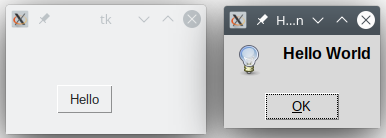
\includegraphics[width=\linewidth]{./gfx/tk-button}
\end{center}
State after clicking the button with label \emph{Hello}.
\end{tcolorbox}
\end{tcbraster}
%
\end{frame}

% =========================================================================== %

\begin{frame}[fragile]{Analysis}
%
\begin{itemize}
\item Load all classes from module tkinter as well as submodule \texttt{messagebox}
\item Define Main window
\item Change shape: \inPy{top.geometry("200x100")}
	\begin{itemize}
	\item Method \texttt{geometry} takes string argument giving size (and window position)
	\item \inPy{"[width]x[height] + [distance from top] + [distance from left]"}
	\item last two elements can be omitted
	\end{itemize}
\item Define secondary elements \enquote{under} \texttt{top}: \inPy{B = tk.Button(top, ...)}
	\begin{itemize}
	\item First Argument: Parent widget
	\item Subsequent arguments: widget-specific
	\item Commonly: \texttt{command = ...} -- callback function
	\end{itemize}
\item Callback function
	\begin{itemize}
	\item Code to be executed when widget is triggered
	\item Signature (expected arguments, return value) depend on widget (usually no arguments and return \inPy{None})
	\item Prepare to look up definitions a lot (\eg online)
	\end{itemize}
\item For optional arguments: see link: {\scriptsize \url{https://www.tutorialspoint.com/python3/tk_button.htm}}
\end{itemize}
%
\end{frame}

% =========================================================================== %

\begin{frame}[fragile]{Other Ways of Aranging Widgets}
%
\begin{itemize}
\item Frames
	\begin{itemize}
	\item Widgets, invisible Boxes
	\item Other widgets can be children of frames
	\item Groups for automatic arrangement
	\end{itemize}
\item Method \texttt{pack} of all widgets
	\begin{itemize}
	\item (Re-)positions all widgets in container
	\item Possibly resizes other widgets
	\item Aims for equal space for everything
	\item Optional Parameters
		\begin{itemize}
		\item \inPy{expand=True} -- make packed widget(s) occupy maximum space
		\item \inPy{fill=None} -- refinement of \texttt{expand} option: expand only in width (\texttt{tk.X}), height (\texttt{tk.Y}) or \texttt{tk.BOTH}
		\item \inPy{side=tk.TOP} -- from where to \enquote{push in} the new widget. Alternatives: \texttt{tk.BOTTOM}, \texttt{tk.LEFT}, \texttt{tk.RIGHT}
		\item \inPy{side=tk.TOP}, etc. are actually only strings, holding \inPy{"top"}, ...
		\end{itemize}
	\end{itemize}
\item See Link: {\scriptsize \url{https://www.tutorialspoint.com/python3/tk_pack.htm}}
\end{itemize}
%
\end{frame}

% =========================================================================== %

\begin{frame}[fragile]
%
\begin{minipage}{.49\linewidth}
\begin{codebox}[Example: Buttons and Frames...]
\begin{minted}[fontsize=\scriptsize, linenos]{python3}
import tkinter as tk

root  = tk.Tk()

topframe = tk.Frame(root)
topframe.pack()

bottomframe = tk.Frame(root)
bottomframe.pack(
  side = tk.BOTTOM,
  fill = tk.X)

redbutton = tk.Button(
  topframe,
  text = "Red", fg = "red")
redbutton.pack(side = tk.LEFT)

greenbutton = tk.Button(
  topframe,
  text = "Green", fg = "green")
greenbutton.pack(side = tk.LEFT)
\end{minted}
\end{codebox}
\end{minipage}
%
\begin{minipage}{.49\linewidth}
\begin{codebox}[... Continued]
\begin{minted}[fontsize=\scriptsize, linenos, firstnumber=last]{python3}
bluebutton = tk.Button(
  topframe,
  text = "Blue", fg = "blue")
bluebutton.pack(side = tk.LEFT)

blackbutton = tk.Button(
  bottomframe,
  text = "Black", fg = "black")
blackbutton.pack(
  side = tk.BOTTOM, fill = tk.X)

root.mainloop()
\end{minted}
\end{codebox}
\begin{tcolorbox}[title=Output: Buttons and Frames]
\begin{center}
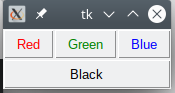
\includegraphics[width=.49\linewidth]{./gfx/tk-buttonsframe}
\end{center}
\end{tcolorbox}
\end{minipage}
%
\end{frame}

% =========================================================================== %

\begin{frame}[fragile]
%
\begin{columns}[T]
\column{.5\linewidth}
\begin{Large}
	{Other Ways of Aranging Widgets}
%	\vspace{6pt}
\end{Large}
\begin{itemize}
\item Method \texttt{grid}
	\begin{itemize}
	\item Arrange widgets on a grid
	\item Optional arguments \texttt{row} and \texttt{col} -- integers defining position
	\item Grid is automatically resized for each added element
	\item More optional parameters: {\scriptsize \url{https://www.tutorialspoint.com/python3/tk_grid.htm}}
	\end{itemize}
\end{itemize}
\begin{center}
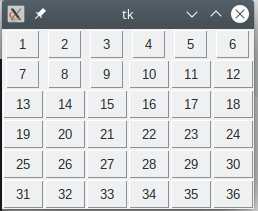
\includegraphics[width=.35\linewidth]{./gfx/tk-grid}
\end{center}
%
\column{.5\linewidth}
\begin{codebox}[Example: \texttt{grid}]
\begin{minted}[fontsize=\scriptsize, linenos]{python3}
import tkinter as tk
root = tk.Tk()

lbl = 0
for r in range(6):
   for c in range(6):
      lbl = lbl + 1
      tk.Button(
          root, 
          text = str(lbl),
          borderwidth = 1
      ).grid(
          row    = r,
          column = c
      )

root.mainloop()
\end{minted}
\end{codebox}
\end{columns}
%
\end{frame}

% =========================================================================== %

\begin{frame}[fragile]{Widgets with States -- Variable-Mechanism}
%
\begin{itemize}
\item Widgets like checkbuttons, radiobuttons, ...: state
	\begin{itemize}
	\item checked/unchecked, option x/y, ...
	\end{itemize}
\item Access via external variable (\ie no read/write methods available for all widgets)
\item Like callback-Function: optional argument \texttt{variable = ...}
\item Variable is an instance of one of several tk-classes
	\begin{itemize}
	\item \texttt{tk.IntVar} -- stores an \inPy{int}, default for checkbuttons and radiobuttons
	\item \texttt{tk.StringVar} -- stores \inPy{str}ings
	\item Updates to these variables will directly affect linked controls
	\item (This is why extra classes are needed)
	\end{itemize}
\end{itemize}
%
\end{frame}

% =========================================================================== %

\begin{frame}[fragile]
%
\begin{tcbraster}[raster columns=2,
                  raster equal height,
                  nobeforeafter,
                  raster column skip=0.5cm]
\begin{codebox}[Example: Two Checkbuttons ...]
\begin{minted}[fontsize=\scriptsize, linenos]{python3}
import tkinter as tk

top = tk.Tk()

CheckVar1 = tk.IntVar()
CheckVar2 = tk.IntVar()

def getChoiceText () :
  reVal = ""
  if CheckVar1.get() == 1 and \
     CheckVar2.get() == 1 :
    reVal = "Music and Video"
  elif CheckVar1.get() == 1 :
    reVal = "Music only"
  elif CheckVar2.get() == 1 :
    reVal = "Video only"
  else :
    reVal = "Nothing"
  return reVal
\end{minted}
\end{codebox}
%
\begin{codebox}[... Continued]
\begin{minted}[fontsize=\scriptsize, linenos, firstnumber=last]{python3}
chk1 = tk.Checkbutton(
    top,
    text = "Music",
    variable = CheckVar1)
chk1.pack()

chk2 = tk.Checkbutton(
    top,
    text = "Video",
    variable = CheckVar2)
chk2.pack()

btn = tk.Button(
    top,
    text = "Print Choice",
    command = lambda : 
        print(getChoiceText()) )
btn.pack()

top.mainloop()
\end{minted}
\end{codebox}
\end{tcbraster}
%
\end{frame}

% =========================================================================== %

\begin{frame}[fragile]
%
\begin{tcbraster}[raster columns=2,
                  raster equal height,
                  nobeforeafter,
                  raster column skip=0.5cm]
\begin{codebox}[Example: Radiobuttons ...]
\begin{minted}[fontsize=\scriptsize, linenos]{python3}
import tkinter as tk

top = tk.Tk()
rows = 5

optionL = tk.IntVar()
optionR = tk.IntVar()

getChoiceText = lambda : 
    chr(optionL.get() + 65) + \
    str(optionR.get())

for i in range(rows) :
    tk.Radiobutton(
        text=chr(i + 65),
        variable=optionL,
        val=i
    ).grid(
        row=i, column=0
    )
\end{minted}
\end{codebox}
%
\begin{codebox}[... Continued]
\begin{minted}[fontsize=\scriptsize, linenos, firstnumber=last]{python3}
for i in range(rows) :
    tk.Radiobutton(
        text=str(i),
        variable=optionR,
        val=i
    ).grid(
        row=i, column=1
    )

tk.Button(
    text="Print Choice",
    command = lambda :
        print( getChoiceText() )
).grid(
    row=rows, column=0,
    columnspan=2
)

top.mainloop()
\end{minted}
\end{codebox}
\end{tcbraster}
%
\end{frame}

% =========================================================================== %

\begin{frame}[fragile]{Textboxes}
%
%
\begin{itemize}
\item Class \texttt{tk.Entry} -- one line textbox
	\begin{itemize}
	\item \emph{Compatible} with \texttt{variable} mechanism
	\item Would then take an \texttt{tk.StringVar}
	\item Not strictly necessary (but sometimes convenient)
	\item Callback \texttt{command} called each time the state changes (each keypress)
	\item String \texttt{show} -- hide typed characters (for passwords)
	\item See link: {\scriptsize \url{https://www.tutorialspoint.com/python3/tk_entry.htm}}
	\end{itemize}
\item Class \texttt{tk.Text} -- multiline textbox
	\begin{itemize}
	\item Similar attributes
	\item No \texttt{show} feature
	\item Rich Text Capacity -- \eg coloured text
	\item See link: {\scriptsize \url{https://www.tutorialspoint.com/python3/tk_text.htm}}
	\end{itemize}
\end{itemize}
%
\end{frame}

% =========================================================================== %

\begin{frame}[fragile]
%
\begin{tcbraster}[raster columns=2,
                  raster equal height,
                  nobeforeafter,
                  raster column skip=0.5cm]
\begin{codebox}[Example: Entries...]
\begin{minted}[fontsize=\scriptsize, linenos]{python3}
import tkinter as tk

top = tk.Tk()

frametop = tk.Frame(top)
frametop.pack(side=tk.TOP)

framebtm = tk.Frame(top)
framebtm.pack(side=tk.BOTTOM, fill=tk.X)

L1 = tk.Label(frametop,
              text = "User Name"
)
L1.pack(side = tk.LEFT)
\end{minted}
\end{codebox}
%
\begin{codebox}[... Continued]
\begin{minted}[fontsize=\scriptsize, linenos, firstnumber=last]{python3}
E1 = tk.Entry(frametop)
E1.pack(side = tk.RIGHT)

B1 = tk.Button(
    framebtm,
    text="show",
    command = lambda : print(E1.get())
)
B1.pack(fill=tk.X)

top.mainloop()
\end{minted}
\end{codebox}
\end{tcbraster}
%
%\begin{tcolorbox}[title=Output: Buttons and Frames]
\begin{center}
	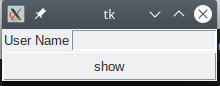
\includegraphics[width=.25\linewidth]{./gfx/tk-entry}
\end{center}
%\end{tcolorbox}
%
\end{frame}

% =========================================================================== %

\begin{frame}[fragile]{Listboxes}
%
\begin{itemize}
\item Select one or multiple strings out of a list
\item Widget \texttt{tk.Listbox}
	\begin{itemize}
	\item Important Attributes to the Constructor
		\begin{itemize}
		\item \texttt{height} -- number of lines
		\item \texttt{selectmode} -- \texttt{tk.SINGLE} (select one item), \texttt{tk.MULTIPLE} (select several items) or \texttt{tk.EXTEND} (select adjacent items)
		\item \emph{No} command option
		\end{itemize}
	\item Important Methods 
		\begin{itemize}
		\item \texttt{insert(index, string)} -- adds an option
		\item \texttt{delete(index)} -- removes an option
		\item \texttt{activate(index)} -- select one item
		\item \texttt{curselection()} -- returns \inPy{tuple} of selected lines (or empty \inPy{tuple})
		\item \texttt{get(index)} -- returns in line \texttt{index}. \texttt{index} can be a \inPy{tuple}, too.
		\end{itemize}
	\end{itemize}
\end{itemize}
%
\end{frame}

% =========================================================================== %

\begin{frame}[fragile]
%
\begin{columns}[T]
\column{.5\linewidth}
\begin{Large}
	{Example: Listboxes}
	\vspace{12pt}
\end{Large}
%
\begin{itemize}
\item Aim: Buttons add predefined lines to Listbox
\item Button \texttt{>} adds user text to listbox
\item Button \texttt{remove} deletes a selected line from listbox
\item Button \texttt{order} displays listbox content and terminates the program
\end{itemize}
%
\column{.5\linewidth}
\begin{tcolorbox}[title=Pizza Order Tool]
\begin{center}
	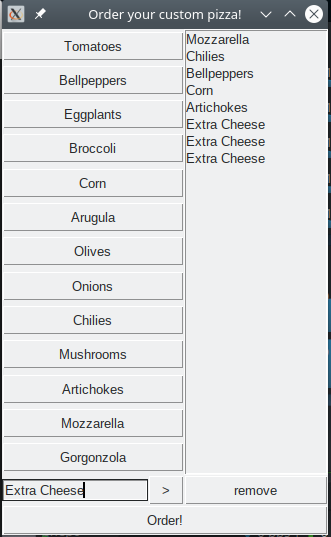
\includegraphics[width=.5\linewidth]{./gfx/tk-listbox}
\end{center}
\end{tcolorbox}
\end{columns}
%
\end{frame}

% =========================================================================== %

\begin{frame}[fragile]
%
\begin{codebox}[Example: Pizza Order Tool (1)]
\begin{minted}[linenos, fontsize=\scriptsize]{python3}
import tkinter as tk
import tkinter.messagebox as msg

defaultOptions = ("Tomatoes", "Bellpeppers", "Eggplants", "Broccoli", "Corn",
                  "Arugula", "Olives", "Onions", "Chilies", "Mushrooms",
                  "Artichokes", "Mozzarella", "Gorgonzola")

# numerical constants: describe width and height of the interface
N = len(defaultOptions)
W = 6

top = tk.Tk()
top.title("Order your custom pizza!")

buttons = []
for i, ingredient in enumerate(defaultOptions) :
    buttons.append(tk.Button(
        top,
        text = ingredient,
        command = lambda c=i: lst.insert(tk.END, buttons[c]["text"])
    ))
\end{minted}
\end{codebox}
%
\end{frame}

% =========================================================================== %

\begin{frame}[fragile]
%
\begin{codebox}[Example: Pizza Order Tool (2)]
\begin{minted}[linenos, fontsize=\scriptsize, firstnumber=last]{python3}
    buttons[i].grid(
        column = 0, row = i,
        columnspan = W,     # use W cells in the grid
        sticky = "WE"       # fill the entire width of the grid
    )

txt = tk.Entry (top)
txt.grid(
    column = 0, row = N,
    columnspan = W - 1
)

tk.Button(
    top,
    text = ">",
    command = lambda : lst.insert(tk.END, txt.get())
).grid(column = W - 1, row = N)

lst = tk.Listbox(top, height = 2*N)
lst.grid(column = W + 1, row = 0, rowspan=N)
\end{minted}
\end{codebox}
%
\end{frame}

% =========================================================================== %

\begin{frame}[fragile]
%
\begin{codebox}[Example: Pizza Order Tool (3)]
\begin{minted}[linenos, fontsize=\scriptsize, firstnumber=last]{python3}
tk.Button(
    top,
    text = "remove",
    command = lambda :
        lst.delete(*lst.curselection()) if len(lst.curselection()) else None
).grid(
    column = W + 1, row = N,
    sticky = "WE"
)

def getOrderText () :
    reVal = "One pizza with"
    if lst.size() == 0 :
        reVal += " nothing"
    else :
        for ID in range(lst.size()) :
            reVal += "\n* " + lst.get(ID)
    return reVal
\end{minted}
\end{codebox}
%
\end{frame}

% =========================================================================== %

\begin{frame}[fragile]
%
\begin{codebox}[Example: Pizza Order Tool (4)]
\begin{minted}[linenos, fontsize=\scriptsize, firstnumber=last]{python3}
def orderMsgBox () :
    msg.showinfo("your Order", getOrderText())
    top.destroy()    # closes the main window

tk.Button(
    top,
    text = "Order!",
    command = orderMsgBox
).grid(
    column = 0, row = N + 1,
    columnspan = W + 2,
    sticky = "WE"
)

top.mainloop()
\end{minted}
\end{codebox}
%
\end{frame}

% =========================================================================== %

\begin{frame}[fragile]{Pre-Built Dialogs}
%
\begin{itemize}
\item Module \texttt{tk.filedialog} -- load file / save file / select directory dialogs
\item Module \texttt{tk.colorchooser} -- get hex colour value from user
\item Module \texttt{tk.messagebox} -- different Symbols and pre-defined buttons
\item All of them: See \url{https://tkdocs.com/tutorial/windows.html#dialogs}
\end{itemize}
%
\begin{hintbox}[Have a look around]
This lecture has, again, only shown you a fraction of what tkinter can do.

Browse the links provided to see which widgets are supported and how they behave. Use your search engine of choice to find example codes on many a scenario.
\end{hintbox}
%
\end{frame}
